\documentclass[10 pt, twocolumn]{article}

\usepackage[utf8]{inputenc}
\usepackage[T1]{fontenc}
\usepackage{caption}
\usepackage{graphicx}
\usepackage{xcolor}
\usepackage{interval}
\usepackage{listingsutf8}
\usepackage{hyperref}
\usepackage{siunitx}
\usepackage{algorithm2e}
\usepackage{rotating}
\usepackage{adjustbox}
\usepackage{booktabs}
\usepackage{pgfplots}
\usepackage{tikz}
\usepackage{footmisc}
\usepackage{amsfonts}
\usepackage[backend=biber,style=numeric]{biblatex}
\usepackage[
  left=1.50cm,
  right=1.50cm,
  top=2.00cm,
  bottom=2.00cm
]{geometry}

\pgfplotsset{compat=1.15}

\sisetup{load-configurations=abbreviations, binary-units=true}
\intervalconfig {
    soft open fences ,
    separator symbol =; ,
}

\lstdefinelanguage{JavaScript}{
  keywords={break, case, catch, continue, debugger, default, delete, do, else, finally, for, function, if, in, instanceof, new, return, switch, this, throw, try, typeof, var, void, while, with},
  morecomment=[l]{//},
  morecomment=[s]{/*}{*/},
  morestring=[b]',
  morestring=[b]",
  sensitive=true
}

\lstdefinelanguage{Protobuf}{
  keywords={message, string, uint32, int32},
  morecomment=[l]{//},
  morecomment=[s]{/*}{*/},
  morestring=[b]',
  morestring=[b]",
  sensitive=true
}

\lstset{
    language=C,
    keywordstyle={\bfseries},
    basicstyle=\footnotesize,
    literate={->}{$\rightarrow{}$}{1} {<-}{$\leftarrow{}$}{1},
    stringstyle=\color{purple},
    keepspaces=true,
    captionpos=b,
    inputencoding=utf8,
    escapeinside={\%*}{*)}
}

\renewcommand\AlCapSty{\text}
\SetAlCapNameFnt{\footnotesize}
\SetAlCapFnt{\footnotesize}
\SetAlgoCaptionSeparator{.}
\DeclareCaptionLabelFormat{nospace}{#1 #2}
\captionsetup[table]{labelformat=nospace,labelfont=rm,name=Table,labelsep=period}

\newcommand{\pcode}[1]{
    \lstinline[basicstyle=\itshape,keywordstyle={}]{#1}
}

\newcommand*{\lstnumberautorefname}{line}

\newcommand{\icode}[1]{\lstinline{#1}}

\newcommand{\name}[1] {\emph{#1}}

\newcolumntype{R}[2]{%
    >{\adjustbox{angle=#1,lap=\width-(#2/2)}\bgroup}%
    l%
    <{\egroup}%
}
\newcommand*\rot{\multicolumn{1}{R{90}{1em}}}

\newcommand{\fig}[3]{
  \begin{figure}[h]
    \begin{center}
        \includegraphics[width=8cm,keepaspectratio]{#1}
        \caption{#3}
        \label{fig:#2}
    \end{center}
  \end{figure}
}

\usepackage[most]{tcolorbox}
\newcounter{example}
\usepackage{xparse}
\usepackage{lipsum}

\def\exampletext{Example} % If English
\NewDocumentEnvironment{example}{ O{} }
{
\colorlet{colexam}{red!55!black} % Global example color
\newtcolorbox[use counter=example]{examplebox}{%
    % Example Frame Start
    empty,% Empty previously set parameters
    title={#1},% use \thetcbcounter to access the example counter text
    % Attaching a box requires an overlay
    attach boxed title to top left,
       % Ensures proper line breaking in longer titles
       minipage boxed title,
    % (boxed title style requires an overlay)
    boxed title style={empty,size=minimal,toprule=0pt,top=4pt,left=3mm,overlay={}},
    coltitle=colexam,fonttitle=\bfseries,
    before=\par\medskip\noindent,parbox=false,boxsep=0pt,left=3mm,right=0mm,top=2pt,breakable,pad at break=0mm,
       before upper=\csname @totalleftmargin\endcsname0pt, % Use instead of parbox=true. This ensures parskip is inherited by box.
    % Handles box when it exists on one page only
    overlay unbroken={\draw[colexam,line width=.5pt] ([xshift=-0pt]title.north west) -- ([xshift=-0pt]frame.south west); },
    % Handles multipage box: first page
    overlay first={\draw[colexam,line width=.5pt] ([xshift=-0pt]title.north west) -- ([xshift=-0pt]frame.south west); },
    % Handles multipage box: middle page
    overlay middle={\draw[colexam,line width=.5pt] ([xshift=-0pt]frame.north west) -- ([xshift=-0pt]frame.south west); },
    % Handles multipage box: last page
    overlay last={\draw[colexam,line width=.5pt] ([xshift=-0pt]frame.north west) -- ([xshift=-0pt]frame.south west); },%
    }
\begin{examplebox}}
{\end{examplebox}\endlist}

\newcommand*\circled[1]{\tikz[baseline=(char.base)]{
            \node[shape=circle,draw,inner sep=1pt] (char) {#1};}}

\usepackage{tikz}

\newcommand{\smiley}{\tikz[baseline=-0.75ex,black]{
    \draw circle (2mm);
\node[fill,circle,inner sep=0.5pt] (left eye) at (135:0.8mm) {};
\node[fill,circle,inner sep=0.5pt] (right eye) at (45:0.8mm) {};
\draw (-145:0.9mm) arc (-120:-60:1.5mm);
    }
}

\newcommand{\frownie}{\tikz[baseline=-0.75ex,black]{
    \draw circle (2mm);
\node[fill,circle,inner sep=0.5pt] (left eye) at (135:0.8mm) {};
\node[fill,circle,inner sep=0.5pt] (right eye) at (45:0.8mm) {};
\draw (-145:0.9mm) arc (120:60:1.5mm);
    }
}

\newcommand{\neutranie}{\tikz[baseline=-0.75ex,black]{
    \draw circle (2mm);
\node[fill,circle,inner sep=0.5pt] (left eye) at (135:0.8mm) {};
\node[fill,circle,inner sep=0.5pt] (right eye) at (45:0.8mm) {};
\draw (-135:0.9mm) -- (-45:0.9mm);
    }
}


\addbibresource{root.bib}

\title{So you want to build a ML system}

\author{Jan Macháček}

\begin{document}

\twocolumn[
  \begin{@twocolumnfalse}
    \maketitle
    \begin{abstract}
      Amongst other things, a machine learning system should be built! It can solve anything, there are so many wonderful frameworks, so many conference talks that show just how easy it is to throw together just a few line of Python, and hey presto!--a machine that can recognise digits in images, recognise hot dog and \emph{not} hot dog... it even runs on a mobile phone. This essay is about the difficulties that are lurking in the execution and running of a robust \& mature machine learning system.
    \end{abstract}
  \end{@twocolumnfalse}
]

\section{What can ML do?}
The exercise analysis system sets out to be a computerized personal for resistance or strength exercise. Exercise systems collect heart rate data as the baseline indication of physical exertion. Depending on the chosen sport, the systems typically collect GPS and accelerometer data. Geolocation, acceleration, and heart rate are fairly comprehensive source of data for outdoors sports: think running or cycling. For cycling, geolocation sampled at, say, \SI{50}{\hertz} reliably establishes the route ridden, but is also the source of data for speed and acceleration; with underlying elevation data \& the weight of the rider and the bicycle, it is possible to estimate power output. With the heart rate, it is possible to get a  fairly accurate view of the activity in \autoref{fig:cycling-overall}.

\fig{cycling-overall.png}{cycling-overall}{An afternoon ride}

In addition to the post-ride analysis, the sensors provide immediate feedback during the ride. A modern cycling computer records and displays speed, elevation, distance, heart rate, pedalling cadence, and power. An athlete can use these values to inform his or her training; for example, one might train for a time trial aiming for a particular power output over a specific distance and use the values a cycling computer displays to guide the training sessions. (See \autoref{fig:cycling-power-training}.)

\fig{cycling-power-training.jpg}{cycling-power-training}{Cycling power training}

Everything becomes much more difficult indoors; and then even more difficult when not in a swimming pool, on a rowing machine, or on a spinning bike; when the user turns to resistance exercise. Some exercise machines now come with Bluetooth ``beacons'' that advertise the details of the activity. Any sensors are less likely to be embedded in free weights (and even if there were sensors, the sensors cannot reveal the exercise the user is performing; though identification such as \SI{20}{\kg} dumbbell is useful, and acceleration \& rotation is even more useful). There are no machines involved at all in body-weight exercises. 

To build a system for resistance exercise analysis that ``matches'' the features of a cycling system \emph{without requiring super high-tech gym}, it will be necessary for the users to \emph{bring their own sensors}. A smartwatch can provide acceleration, rotation, and heart rate\footnote{Though most smartwatches report ``beats per minute'', the watch measures changes of the blood flow velocity, which is directly correlated to heart rate. Nevertheless, the watch does not measure heart rate itself.}; these three sensor readings can be fused with sensor readings from a smartphone that the user might wear in his or her pocket. This gives additional acceleration and rotation. Unfortunately, heart rate lags behind any exertion, so it'll only increase by the time the user is done with a set of a particular exercise (assuming the exercise is done with appropriate intensity); the last easily accessible sensor, geolocation (if at all available due to the location of the exercise floor) will show that the user is not moving much. This leaves only the acceleration and rotation values as useful indications of the movement being performed. 

A proof-of-concept application that allows the users to wear a sensor on their wrists and use their mobile phones to \emph{mark the start and end of each exercise}, together with \emph{the name of the exercise} provides the data to build \& verify the first models. 

\fig{exercise-a.png}{exercise-a}{Two exercises}

\autoref{fig:exercise-a} shows the acceleration from a watch worn on the left wrist. The acceleration is along the $x$, $y$, and $z$ axes (with the Earth contributing \SI{9.8}{\meter\second^{-2}}) sampled at \SI{50}{\hertz}; exercise \circled{1} is the straight bar biceps curl, and \circled{2} is the chest dumbbell flyes. You--the readers, humans--can work out the number of repetitions and you can clearly spot that these are two different exercises, and if you saw enough of these figures, you would be able to learn to identify the two exercises. It should be possible to implement a function \pcode{classify(sensor data) -> exercise} that does the same. Even if this function performs perfectly (i.e. it identifies the movement that corresponds to the exercise for every \pcode{sensor data} that matches the exercise, even if the exact \pcode{sensor data} was not in the training set), it will struggle to identify areas of no exercise; unfortunately no exercise does not mean no movement, it simply means that the user is walking from one machine to another, setting up for a different exercise, taking a drink, and so on. These no exercise areas are quite often also areas of repetitive motion (walking) or fairly large movements (setting up); see \autoref{fig:exercise-vs-slacking} where the red shaded areas represent exercise and the rest is other recorded motion.

\fig{exercise-vs-slacking.png}{exercise-vs-slacking}{Exercise vs. slacking}

The figure shows some of the typical challenges of noisy, mislabelled, and unclensed data. For example in \circled{1}, the user has done two exercise sets, but forgot to label the no exercise area properly. The area in \circled{2} shows large movement in the no exercise section--in this particular example, the acceleration actually shows the user dragging an exercise bench. In \circled{3}, the labelling is not entirely accurate: the user started the label before actually starting the exercise. Finally, \circled{4} shows further wide movements in the no exercise section. To deal with the complexity of exercise and no exercise, the classification function needs to be \pcode{classify(sensor data) -> result}, where \pcode{result = exercise | no-exercise}. 

\subsection{Sensors are not enough}
Suppose there is indeed a function that takes the sensor readings and returns the details of the exercise being performed: \pcode{classify(sensor data) -> result}. Even if this function performs perfectly, it only allows to build a system that lags behind the users' movement. Even if the system could read the data from the sensors with zero delay, the system would only be able to tell the user what he or she is doing after ``seeing'' some minimum amount of data, introducing lag. High lag will cause the user experience to be rather frustrating. In our testing, a \SI{100}{\milli\second} lag is noticeable; \SI{250}{\milli\second} lag is still tolerable; anything over \SI{750}{\milli\second} is downright confusing. A good example is the number of repetitions: with an exercise whose single repetition takes around \SI{1}{\second}, a \SI{750}{\milli\second} lag will mean that the system shows 5\textsuperscript{th} repetition when in fact the user is starting on his or her 7\textsuperscript{th}. Compare this to the sensor readings that the cycling computer reports: speed, altitude and similar can be reported as they are measured (typically a few times per second); cadence and power readings usually lag behind the instantaneous measurements because the computers display average values over a short time window. Just like the repetitions in resistance exercise, the lag is confusing; though if the athlete holds fairly steady power output, the reading usually matches the percieved effort.

The machine learning resistance exercise system is competing with a simple exercise log on paper notebook. Following users that use such an \emph{ancient} technology reveals the flow that the application has to satisfy. 

To understand what the users expect from an intuitive application, it is necessary

\section{The complexity of sensors}
The system reads values from the sensors; the values are not read continuously, but read at discrete points in time. The range of sensor values can introduce clipping errors, and the sampling rate can introduce aliasing errors. Good choice of sampling rate and sensor types can reduce these errors: both sampling rates and sensor value range must be significantly greater than expected measurements; even in that case, the system must include enough signal processing to eliminate rogue values. For humans in resistance exercise, the sampling rate is sufficient to be \SI{50}{\hertz}, acceleration is expected to be in the range \SI{\pm40}{\meter\second^{-2}}, rotation \SI{\pm4\pi}{\radian\second^{-1}}. The first stab at implementing the sensor reading code may take the form of a loop in \autoref{alg:naive-sensor-sampling}.

\begin{algorithm}
  \caption{Simple sensor sampling}
  \label{alg:naive-sensor-sampling}
  \DontPrintSemicolon
  \SetKw{Emit}{emit}
  \SetKwFunction{sensor}{sensor}
  \SetKwFunction{currentValue}{currentValue}
  \SetKwFunction{sleep}{sleep}
  $acc \leftarrow$ \sensor{type = accelerometer}\;
  $gyro \leftarrow$ \sensor{type = gyroscope}\;
  \BlankLine
  \While{true}{
    \sleep{interval = $\SI{20}{\milli\second}$}\;
    $a \leftarrow $ $acc$.\currentValue{}\;
    $r \leftarrow $ $gyro$.\currentValue{}\;
    \Emit{$a, r$}\;
  }
\end{algorithm} 

When implemented in real hardware, this algorithm suffers from \emph{timing errors} as well as \emph{high power consumption}. When it comes to reading the samples, is it acceptable to read acceleration before rotation?; moreover the act of obtaining those samples adds time, which means that the \SI{20}{\milli\second} in the $sleep$ is too long, but \SI{19}{\milli\second} is too short. The infinite loop with the \pcode{sleep} syscall prevents the CPU from slowing down into more power-efficient modes. Modern hardware typically provides a way to begin the sensor readings, with the sensors storing the samples (pairs of \pcode{timestamp -> value}) in a memory buffer without any interaction from the user program, and provide a way to access sections of the buffer at arbitrary intervals. (Viz \autoref{alg:async-sensor-sampling}.)

\begin{algorithm}
  \caption{Asynchronous sensor sampling}
  \label{alg:async-sensor-sampling}
  \SetKwProg{Fn}{Function}{ is}{end}
  \SetKwFunction{sensor}{sensor}
  \SetKwFunction{start}{start}
  \SetKwFunction{timer}{timer}
  \SetKwFunction{bufferedValuesSince}{bufferedValuesSince}
  \SetKwFunction{fuse}{fuse}
  \SetKw{Emit}{emit}
  \DontPrintSemicolon
  $acc \leftarrow$ \sensor{type = accelerometer}\;
  $gyro \leftarrow$ \sensor{type = gyroscope}\;
  $timestamp \leftarrow DistantPast$\;
  $timerFun \leftarrow$ \Fn{}{
    $A \leftarrow$ $acc$.\bufferedValuesSince{timestamp}\;
    $R \leftarrow$ $gyro$.\bufferedValuesSince{timestamp}\;
    $S, timestamp \leftarrow$ \fuse{A, R}\;
    \Emit{S}\;
  }
  $timer \leftarrow$ \timer{callback = timerFun}\;
  \BlankLine
  Start: \Begin{
    $acc$.\start{rate = $\SI{50}{\hertz}$}\;
    $gyro$.\start{rate = $\SI{50}{\hertz}$}\;
    $timer$.\start{interval = $\SI{500}{\milli\second}$}\;
  }
\end{algorithm} 

This approach addresses the high power consumption, as well as some of the aliasing errors in \autoref{alg:naive-sensor-sampling}. However, the sample buffers read from the sensors are not always precisely aligned with respect to wall time (i.e. time as measured by a [precise] clock on a wall) and might even contain gaps where the sensor wasn't able to obtain a value. \autoref{plot:timing-errors} shows sample buffers obtained from two sensors sampled at \SI{50}{\hertz}: the values should be exactly \SI{20}{\milli\second} apart, and the sample buffers from the two sensors should begin at the same wall time. Unfortunately, the available sensors (and their operating systems / runtimes) usually result in the sample buffers not beginning at the same wall time; similarly, the timestamps of the values in the buffers will not necessarily fall precisely on integer multiples of the sampling period.

\begin{figure}[ht]
  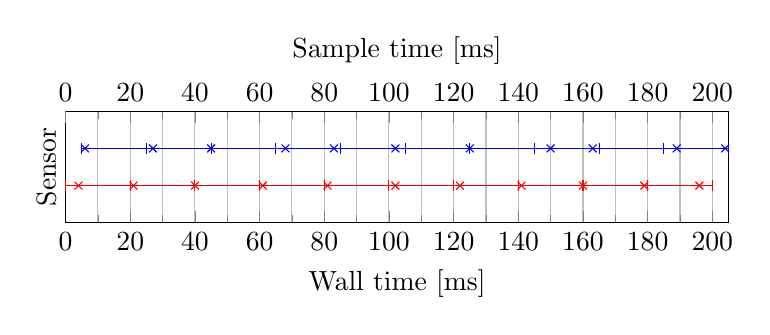
\begin{tikzpicture}
    \begin{axis}[
      height=3cm, 
      width=10cm, 
      xminorgrids=true,
      xmajorgrids=true,
      xlabel={Wall time [ms]}, 
      ylabel={Sensor},
      ytick=\empty,
      yticklabels=\empty,
      xmin=0,xmax=205,
      ymin=0,ymax=3,
      minor tick num=1,
      legend pos=south east,
      legend cell align={left}
      ]

      \addplot[color=red,mark=|] coordinates {
        (0,   1) 
        (20,  1)
        (40,  1)
        (60,  1)
        (80,  1)
        (100, 1)
        (120, 1)
        (140, 1)
        (160, 1)
        (180, 1)
        (200, 1)
      };
      \addplot[color=blue,mark=|] coordinates {
        (5,   2)
        (25,  2)
        (45,  2)
        (65,  2)
        (85,  2)
        (105, 2)
        (125, 2)
        (145, 2)
        (165, 2)
        (185, 2)
        (205, 2)
      };
    \end{axis}
    \begin{axis}[
      height=3cm, 
      width=10cm, 
      xmin=0,xmax=205,
      ymin=0,ymax=3,
      grid=none,
      ytick=\empty,
      yticklabels=\empty,
      minor tick num=1,
      axis x line*=top,
      axis y line=none,
      xlabel={Sample time [ms]}   
    ]
      \addplot[color=red,mark=x] coordinates {
        (4,   1)
        (21,  1)
        (40,  1)
        (61,  1)
        (81,  1)
        (102, 1)
        (122, 1)
        (141, 1)
        (160, 1)
        (179, 1)
        (196, 1)
      };
      \addplot[color=blue,mark=x] coordinates {
        (6,   2)
        (27,  2)
        (45,  2)
        (68,  2)
        (83,  2)
        (102, 2)
        (125, 2)
        (150, 2)
        (163, 2)
        (189, 2)
        (204, 2)
      };
    \end{axis}
  \end{tikzpicture}
  \caption{Timing errors}
  \label{plot:timing-errors}
\end{figure}

The system has to be able to cope with these misalignments and missing values: its goal is to \emph{fuse} the sensors values so that all samples appear as though they were read from a \emph{single reliable} sensor. If the sample buffers differ by less than 1 sample's period the system can simply force the alignment; though it must keep track of the timing error it introduces. If the sample buffers differ by more than 1 sample's period, or if the sample buffer contains \emph{small} gaps, the system should extrapolate the misaligned or missing values. \autoref{fig:sf-gaps} shows the performance of a time-series prediction algorithm applied to gaps of 50 samples--the prediction is fairly accurate in the gaps \circled{1} and \circled{2}, but fails in \circled{3}.

\fig{sf-gaps.png}{sf-gaps}{Extrapolating missing values}

\subsection{Low-power sensors}
sss

\subsection{Security \& Attacks}
\cite{Fu:AuI932n8})

\section{Privacy}

\printbibliography

\end{document} 